\section{Considerações Iniciais}

Nos Capítulo~\ref{chapter:catalogo_refactoring_KDM},~\ref{chapter:Toward_a_Refactoring_Metamodel_for_KDM} e~\ref{chapter:Abordagem_de_sincronizacao} foram apresentadas soluções para auxiliar o engenheiro de modernização a aplicar, reutilizar e propagar refatorações no contexto da abordagem ADM e do metamodelo KDM. Além disso, no Capítulo X foi apresentado uma ferramenta, KDM-RE, que automatiza todo o processo de aplicação, reutilização e propagação de mudanças no contexto do metamodelo KDM, deixando somente sob responsabilidade do engenheiro de software a identificação de onde aplicar refatorações. Desse modo, com o uso da ferramenta o engenheiro de software tem um ambiente totalmente integrado no ambiente Eclipse, onde refatorações podem ser aplicadas e reutilizadas sem se preocupar com a propagação de mudanças para outras visões/artefatos representados em uma determinada instância do metamodelo KDM.

Com o objetivo de verificar se as refatorações adaptadas para o metamodelo KDM realmente melhoraram a qualidade de um sistema e com o intuito de verificar se a ferramenta KDM-RE realmente proporciona facilidade e eficiência na prática, foi-se realizado dois experimentos ao longo deste projeto de doutorado. Esses experimentos foram planejados e executados seguindo a abordagem definida por~\citeonline{Wohlin}, que é composta por três principais fases: (\textit{i}) definição e planejamento, onde são especificados o contexto, as hipóteses, as variáveis, os participantes (quando necessário), os instrumentos e o modelo do experimento; (\textit{ii}) operação, onde ocorre a preparação e a execução do experimento com ou sem os participantes; e (\textit{iii}) análise dos dados, onde os dados coletados durante o experimento são agrupados e analisados por meio de técnicas estatísticas.

Na Seção~\ref{sec:teste_estatisticos} há uma descrição dos testes estatísticos aplicados no experimento realizado durante este projeto de doutorado. Na Seção~\ref{sec:experimento} é descrito o experimento que verifica se as refatorações adaptadas para o metamodelo KDM realmente melhoram a qualidade de um sistema. Na Seção~\ref{sec:experimento_KDM_re} é apresentado um experimento que avaliou a ferramenta KDM-RE. Em seguida, na Seção~\ref{sec:consideracoes_finais_experimento} são comentadas as considerações finais desse capítulo.

\section{Testes Estatísticos}\label{sec:teste_estatisticos}

~\citeonline{Wohlin} declaram que os experimentos têm como objetivo responder questões a respeito de um objeto de estudo. Para cada questão são definidas uma ou mais métricas a partir da qual os dados são coletados e também um conjunto de hipóteses sobre os possíveis resultados são definidos. Esse conjunto de hipóteses é formado por:

\begin{itemize}
\item Uma \textbf{hipótese nula}: Considera que não há uma diferença significativa entre os dados obtidos ao se aplicarem os diferentes tratamentos sobre o objeto de estudo;
\item Uma ou mais \textbf{hipóteses alternativas}: Consideram os demais possíveis resultados. Por exemplo, a hipótese alternativa 1 considera que a ferramenta X é mais eficiente do que a ferramenta Y, enquanto que a hipótese alternativa 2 considerada que a ferramenta X é menos eficiente do que a ferramenta Y.
\end{itemize}

Alguns cálculos podem ser realizados sobre os dados coletados para obter um resultado e uma das hipóteses alternativas ser aceita. Por exemplo, cálculos de média e de porcentagem podem indicar que, em determinado experimento, o tempo gasto pelos participantes para aplicar refatorações no metamodelo KDM foi menor quando a ferramenta X foi utilizada do que quando a ferramenta Y foi utiliza. Contudo, ainda se faz necessários testes estatísticos para comprovar que esse resultado é significativo, refutando assim, a hipótese nula.

No experimento apresentado na Seção~\ref{sec:experimento_KDM_re} foram aplicado os testes estatísticos \textbf{Shapiro-Wilk} e \textbf{Paried T-Test}. Os testes estatísticos foram aplicados com o apoio da ferramenta R\footnote{\texttt{https://www.r-project.org/}}. Esses testes são brevemente explicados a seguir. \change{mudar Colocar os testes estatisticos realmentes utilizados}

\begin{figure}[h]
	\centering
	\caption{Representação gráfica de uma distribuição normal de dados.}
	\label{fig:shapiro_wilk}
	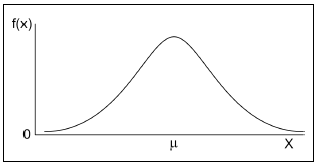
\includegraphics[scale=0.9]{images/distribuicao_normal}
	\fautor
\end{figure}

\subsection{Shapiro-Wilk e Paired T-Test}\label{sec:shapiro_wilk}

O teste \textbf{Shapiro-Wilk} é aplicado para verificar se um conjunto de dados segue, ou não, uma distribuição normal, que possui graficamente o formato de um sino simétrico em relação à sua média, ver Figura~\ref{fig:shapiro_wilk}. Se o p-valor (resultado) do teste \textbf{Shapiro-Wilk} sobre um conjunto de dados for menor do que 0.05 significa que a chance dos dados seguirem uma distribuição normal é menor do que 5\%. Quando esse resultado ocorre, considera-se, estatisticamente, que os dados não seguem uma distribuição normal~\cite{Wohlin}. 


Em geral, as ferramentas de estatísticas utilizam um gráfico de probabilidade, também conhecido como \textit{Q-Q Plot} para representar graficamente a distribuição de um conjunto de dados. Nesse gráfico, quando os dados se posicionam ao redor da linha diagonal, considera-se que os dados seguem uma distribuição normal. Na Figura~\ref{fig:qq_plot_exemple} são apresentados dois exemplos de gráficos de probabilidade, um com distribuição normal e outro não normal.

\begin{figure}[h]
	\centering
	% Requires \usepackage{graphicx}
	\caption{Exemplos de gráficos de probabilidade.}
	\label{fig:qq_plot_exemple}
	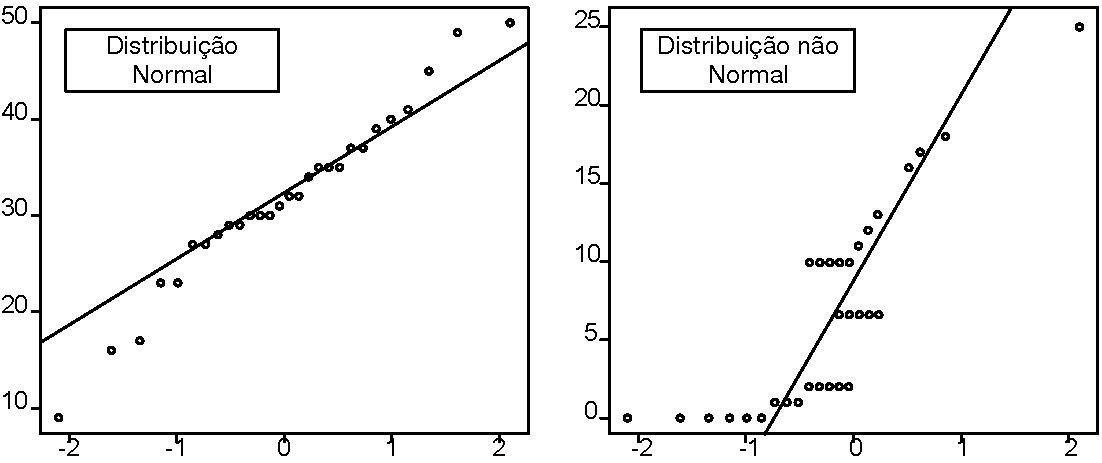
\includegraphics[scale=0.7]{images/qq_plot_exemplo}
	\fautor
\end{figure}

O teste \textbf{Paired T-Test} é utilizado para confrontar dois conjuntos de dados. Esse teste pode ser aplicado somente quando ambos os conjuntos de dados seguem uma distribuição normal. Se o p-valor (resultado) do \textbf{Paired T-Test} for menor que 0.05 significa que a chance dos dois conjuntos de dados serem estatisticamente semelhantes é menor do que 5\%. Portanto, nesse caso, a hipótese nula deve ser rejeitada~\cite{Wohlin}.

\section{Experimento 1: Refatorações no contexto do metamodelo KDM}\label{sec:experimento}

Nesta seção é apresentado um experimento conduzido com o objetivo de analisar as qualidades das refatorações adaptadas para o metamodelo KDM. Especificamente, a seguinte questão de pesquisa é investida nesse experimento:

\textbf{Questão de Pesquisa 1} (\textbf{$QP_1$}): Como as refatorações adaptadas/definidas para o metamodelo KDM podem ser úteis para engenheiros de modernização no cenário do mundo real? O benefício esperado de refatoração não esta limitada apenas à correção de \textit{bad-smells}, mas também podem e devem ser utilizadas para melhorar os atributos de qualidade dos programas, ou seja, melhorar à \aspas{reusabilidade}, \aspas{flexibilidade}, \aspas{facilidade de compreensão} e \aspas{eficácia}.


Dessa forma, para avaliar a \textbf{$QP_1$} sete sistemas foram escolhidos para aplicar um conjunto de refatorações. Esses sete sistemas são bem conhecidos na literatura e estão implementados na linguagem de programação Java: Xerces-J\footnote{\texttt{http://xerces.apache.org/xerces-j/}}, Jexel\footnote{\texttt{https://jexel.googlecode.com}}, JFreeChart\footnote{\texttt{http://www.jfree.org/jfreechart/}}, Jester\footnote{\texttt{jester.sourceforge.net}}, GanttProject\footnote{\texttt{http://www.ganttproject.biz/}}, ArtofIllusion\footnote{\texttt{www.artofillusion.org}} e JHotDraw\footnote{\texttt{jhotdraw.org}}. Xerces-J é uma família de software para analisar (\textit{parsing}) XML. Jexel é API para escrever expressões regulares em Java. JFreeChart é uma biblioteca Java utiliza para gerar gráficos. Jester é uma biblioteca Java utiliza para gerar teste de unidades. GanttProject é uma sistema para gerenciamento de projetos. ArtofIllusion é uma API para modelagem e renderização em 3D. JHotDraw é uma ferramenta para auxiliar a criação de desenhos. Todos os sistemas foram transformados em instâncias do metamodelo KDM utilizando a ferramenta MoDisco\footnote{\texttt{https://eclipse.org/MoDisco/}}. 


\begin{table}[h]
\centering
\caption{Sistemas utilizados no Experimento 1.}
\label{tab:sistemas_experimentos}
\begin{tabular}{ | m{2cm} | m{1cm}| m{1cm}| m{1cm} | m{1cm} | } 
\hline
Sistemas & Siglas & Versão & KLOC & Classes \\ 
\hline
Xerces-J & XJ & 2.7.0 & 240 & 991\\ 
\hline
Jexel & JEX & 1.3 & 50.4 & 75\\
\hline
JFreeChart & JFC & 1.0.9 & 170 & 521\\ 
\hline
Jester & JES & 0.7 & 48 & 14\\ 
\hline
GanttProject & GP & 1.10.2 & 41 & 245\\ 
\hline
ArtofIllusion & AOIL &  2.8.1 & 87 & 459\\ 
\hline
JHotDraw & JHD & 7.0.6 & 16 & 468 \\ 
\hline
\end{tabular}
\end{table}

Na Tabela~\ref{tab:sistemas_experimentos} é possível visualizar algumas informações sobre os sete sistemas. Como apresentado no Capítulo~\ref{chapter:ferramenta_kdm_re}, a ferramenta KDM-RE apenas auxilia o engenheiro de software a aplicar refatorações em instâncias do metamodelo KDM. É de responsabilidade do engenheiro identificar onde aplicar a refatoração uma vez que a ferramenta KDM-RE ainda não identifica \textit{bad-smells}~\cite{Fowler1999}. Assim, esses sete sistemas foram escolhidos, pois na literatura é possível identificar trabalhos que já detectaram e listaram quais são os \textit{bad-smells} desses sistemas e quais são as possíveis refatorações para serem aplicadas como solução~\cite{Kessentini_2011, Ouni_2013, Moha_2010, Kessentini_2010}. Assim, o engenheiro de software apenas precisa aplicar as refatorações nos sistemas.  


Os \textit{bad-smells} identificados nesses sistemas são: \textit{Blob} (uma classe contém muitas linhas de código-fonte e monopoliza o comportamento do sistema), \textit{Data Class} (uma classe que contém apenas atributos, porém não os utilizam para realizar nenhum tipo de processamento), \textit{Spaghetti Code} (código com uma estrutura de controle complexo e emaranhado) e \textit{Functional Decomposition} (quando uma classe desempenha uma única função, ao invés de ser um encapsulamento de dados e funcionalidade)~\cite{Fowler1999}. Está fora do escopo deste capítulo se aprofundar nesses \textit{bad-smells}. Porém, uma lista completa dos \textit{bad-smells} identificados dos sete sistemas escolhidos para esse experimento pode ser visualizada nos artigos~\cite{Kessentini_2011, Ouni_2013, Moha_2010, Kessentini_2010}.

O principal objetivo desse experimento é verificar se após a aplicação de um conjunto de refatorações com base em \textit{bad-smell} já identificados na literatura~\cite{Kessentini_2011, Ouni_2013, Moha_2010, Kessentini_2010} as refatorações adaptadas para o metamodelo KDM melhoraram os sistemas em termos de atributos de qualidade. Os atributos de qualidade foram avaliados utilizando o modelo \sigla{QMOOD}{\textit{Quality Model for Object-Oriented Design}}~\cite{Bansiya_QMOOD}. O QMOOD é um modelo de qualidade para POO que estabelece um modelo hierárquico definido e empiricamente validado para avaliar atributos de qualidade de POO. O uso do modelo QMOOD nesse experimento ocorreu, pois: (\textit{i}) o QMOOD é bastante utilizado na literatura~\cite{Keeffe_2008, Seng_2006, Jensen_2010} para avaliar o efeito de refatoração e (\textit{ii}) o QMOOD define seis atributos de qualidade (\aspas{facilidade de compreensão} (\textit{understandability}), \aspas{eficácia} (\textit{effectiveness}), \aspas{extensibilidade} (\textit{extendibility}), \aspas{reusabilidade} (\textit{reusability}), \aspas{funcionalidade} (\textit{functionality}) e \aspas{flexibilidade} (\textit{flexibility})) que são calculados utilizando 11 métricas~\cite{Bansiya_QMOOD} (ver Tabela~\ref{tab:QMOOD_quality_metrics} e Tabela~\ref{tab:QMOOD_quality_metrics2}). 


Nesse experimento apenas quatro atributos de qualidade foram considerados: \aspas{reusabilidade}, \aspas{flexibilidade}, \aspas{facilidade de compreensão} e \aspas{eficácia}. De acordo com~\citeonline{Bansiya_QMOOD} esses atributos de qualidade podem ser definidos como: 

\begin{itemize}
\item Reusabilidade: Características de POO que permitem que um projeto seja reaplicado para um novo problema sem esforço significativo;
\item Flexibilidade: A capacidade de um projeto ser adaptado para disponibilizar novos recursos;
\item Facilidade de Compreensão: Propriedades do projeto que permitem que seja facilmente aprendido e compreendido. Está relacionado com a complexidade da estrutura do projeto;
\item Eficácia: Capacidade de o projeto obter a funcionalidade e o comportamento desejado, utilizando conceitos e técnicas de POO.
\end{itemize}

O atributo de qualidade \aspas{funcionalidade} foi excluído nesse experimento porque se assume que, por definição, uma refatoração não deve alterar o comportamento/funcionalidade do sistema; em vez disso, apenas altera a estrutura do sistema. Também foi excluído o atributo de qualidade extensibilidade, pois de acordo com~\citeonline{Bansiya_QMOOD} é um atributo de qualidade subjetivo. 

A Tabela~\ref{tab:QMOOD_quality_metrics} apresenta as propriedades de POO e as métricas que foram utilizadas para mensurar as instâncias do metamodelo KDM antes e após a aplicação das refatorações. A Tabela~\ref{tab:QMOOD_quality_metrics2} apresenta os atributos de qualidade e as propriedades definidas por~\citeonline{Bansiya_QMOOD}. Nesse experimento o ganho de qualidade é calculado pela comparação de cada atributo de qualidade antes e após a aplicação de um conjunto de refatorações. Dessa forma, o ganho total da qualidade ($G_{q}$) para cada atributo de qualidade QMOOD pode ser estimado de acordo com a Definição~\ref{def:qmood}

\begin{definicao}\label{def:qmood}
    \textit{$G_{q_{i}} = q'_{i} - q_{i}$ onde $q'_{i}$ e $q_{i}$ representam os valores do atributo de qualidade $i$ antes e após a aplicação das refatorações, respectivamente.}
\end{definicao}

\begin{table}[!h]
\caption{Métricas utilizadas no modelo QMOOD~\cite{Bansiya_QMOOD}.}
\label{tab:QMOOD_quality_metrics}
\begin{center}
\begin{tabular}{ | m{4.2cm} | m{1.4cm}| m{6cm} | } 
\hline
Propriedades de Projeto & Métrica & Descrição \\ 
\hline
Tamanho do Projeto & DSC & Número de classes no projeto \\ 
\hline
Hierarquias & NOH & Número de Hierarquias \\ 
\hline
Abstração & ANA & Média de Ancestrais \\ 
\hline
Encapsulamento & DAM & Métrica de acesso a dados \\ 
\hline
Acoplamento & DCC & Acoplamento direto entre classes \\ 
\hline
Coesão & CAM & Coesão entre os métodos da classe \\ 
\hline
Composição & MOA & Medida de agregação \\ 
\hline
Herança & MFA & Abstração funcional \\ 
\hline
Polimorfismo & NOP & Número de métodos polimórficos \\ 
\hline
Troca de Mensagens & CIS & Tamanho da interface de uma classe \\ 
\hline
Complexidade & NOM & Quantidade de métodos \\ 
\hline
\end{tabular}
\end{center}
\end{table}

\begin{table}[!h]
\caption{Relacionamento de atributos de qualidade X Propriedade no QMOOD~\cite{Bansiya_QMOOD}.}
\label{tab:QMOOD_quality_metrics2}
\begin{center}
\begin{tabular}{ | m{4cm} | m{10cm} |} 
\hline
Atributo de Qualidade & Fórmula com base nas propriedades de projeto  \\ 
\hline
Reusabilidade & -0,25 x DCC + 0,25 x CAM + 0,5 x CIS + 0,5 x DSC  \\ 
\hline
Flexibilidade & 0.25 x DAM - 0.25 x DCC + 0.5 x MOA +0.5 x NOP \\
\hline
Facilidade de Compreensão & -0.33 x ANA + 0.33 x DAM - 0.33 x DCC + 0.33 x CAM -0.33 x NOP + 0.33 x NOM - 0.33 x DSC \\ 
\hline
Eficácia & 0.2 x ANA + 0.2 x DAM + 0.2 x MOA + 0.2 x MFA + 0.2 x NOP \\ 
\hline
\end{tabular}
\end{center}
\end{table}

\subsection{Definição e Planejamento do Experimento 1}

Esse experimento foi planejado utilizando o modelo GQM (\textit{Goal, Question, Metric})~\cite{Wohlin} que é dividido em cinco partes: 

\begin{itemize}
\item \textbf{Objeto de estudo}: o objeto de estudo desse experimento são as refatorações adaptadas para o metamodelo KDM;
\item \textbf{Propósito}: o propósito desse experimento é avaliar as refatorações adaptadas para o metamodelo KDM;
\item \textbf{Perspectiva}: esse experimento esta sendo executado sobre a perspectiva de um pesquisador;
\item \textbf{Qualidade de foco}: o efeito primário sobre investigação nesse experimento são os atributos de qualidade QMOOD. Mais especificadamente os atributos \aspas{reusabilidade}, \aspas{flexibilidade}, \aspas{facilidade de compreensão} e \aspas{eficácia} após a aplicação de um conjunto de refatoração;
\item \textbf{Contexto}: esse experimento foi conduzido utilizando o ambiente de desenvolvimento Eclipse 4.3.2 em uma máquina 2.5 GHz Intel Core i5 com 8GB de memória física executando o sistema operacional Mac OS X 10.9.2.
\end{itemize}


O experimento pode ser resumido utilizando o seguinte \textit{template}~\cite{Wohlin}: \textbf{Analisar} as refatorações adaptadas para o metamodelo KDM; \textbf{com o propósito de} avaliar as refatorações adaptadas; \textbf{com respeito a} \aspas{reusabilidade}, \aspas{flexibilidade}, \aspas{facilidade de compreensão} e \aspas{eficácia}; \textbf{do ponto de vista dos} pesquisadores; \textbf{no contexto de} distintos sistemas.

\subsubsection{Formulação das Hipóteses}



A \mathbf{$QP_1$} foi formalizada em hipóteses. Para cada atributo de qualidade (\aspas{reusabilidade}, \aspas{flexibilidade}, \aspas{facilidade de compreensão} e \aspas{eficácia}) utilizado nesse experimento foi criado hipóteses como apresentado a seguir:

%\aspas{reusabilidade}, \aspas{flexibilidade}, \aspas{facilidade de compreensão} e \aspas{eficácia}

\begin{itemize}

\item \aspas{Reusabilidade}:

\begin{itemize}
\item \textbf{Hipótese Nula} \textbf{$(H1_{0})$}: Não há diferença significativa entre instâncias do metamodelo KDM antes e após a aplicação de um conjunto de refatorações em relação a reusabilidade. Isso pode ser formalizado como: 

\begin{itemize}
\item $H1_{0}$: $\mu_{reusabilidade_{antes}} = \mu_{reusabilidade_{depois}}$
\end{itemize}

\item \textbf{Hipótese Alternativa} \textbf{$(H1_{1})$}: Há diferença significativa entre as instâncias do metamodelo KDM refatorado e a instância do metamodelo KDM não refatorada em relação a reusabilidade. Isso pode ser formalizado como: 

\begin{itemize}
\item $H1_{1}$: $\mu_{reusabilidade_{antes}} \neq \mu_{reusabilidade_{depois}}$;
\end{itemize}
\end{itemize}

\item \aspas{Flexibilidade}:

\begin{itemize}
%segunda hipotese
\item \textbf{Hipótese Nula} \textbf{$(H2_{0})$}: Não há diferença significativa entre instâncias do metamodelo KDM antes e após a aplicação de um conjunto de refatorações em relação a flexibilidade. Isso pode ser formalizado como: 

\begin{itemize}
\item $H2_{0}$: $\alpha_{flexibilidade_{antes}} = \alpha_{flexibilidade_{depois}}$
\end{itemize}

\item \textbf{Hipótese Alternativa} \textbf{$(H2_{1})$}: Há diferença significativa entre as instâncias do metamodelo KDM refatorado e a instância do metamodelo KDM não refatorada em relação a flexibilidade. Isso pode ser formalizado como: 

\begin{itemize}
\item $H2_{1}$: $\alpha_{flexibilidade_{antes}} \neq \alpha_{flexibilidade_{depois}}$;
\end{itemize}
\end{itemize}

\item \aspas{Facilidade de Compreensão}:

\begin{itemize}
%terceira hipotese
\item \textbf{Hipótese Nula} \textbf{$(H3_{0})$}: Não há diferença significativa entre instâncias do metamodelo KDM antes e após a aplicação de um conjunto de refatorações em relação a facilidade de compreensão. Isso pode ser formalizado como: 

\begin{itemize}
\item $H3_{0}$: $\beta_{compreensao_{antes}} = \beta_{compreensao_{depois}}$
\end{itemize}

\item \textbf{Hipótese Alternativa} \textbf{$(H3_{1})$}: Há diferença significativa entre as instâncias do metamodelo KDM refatorado e a instância do metamodelo KDM não refatorada em relação a facilidade de compreensão. Isso pode ser formalizado como: 

\begin{itemize}
\item $H3_{1}$: $\beta_{compreensao_{antes}} \neq \beta_{compreensao_{depois}}$;
\end{itemize}
\end{itemize}

\item \aspas{Eficácia}:
    
    \begin{itemize}
%terceira hipotese
\item \textbf{Hipótese Nula} \textbf{$(H4_{0})$}: Não há diferença significativa entre instâncias do metamodelo KDM antes e após a aplicação de um conjunto de refatorações em relação a eficácia. Isso pode ser formalizado como: 

\begin{itemize}
\item $H4_{0}$: $\gamma_{eficacia_{antes}} = \gamma_{eficacia_{depois}}$
\end{itemize}

\item \textbf{Hipótese Alternativa} \textbf{$(H4_{1})$}: Há diferença significativa entre as instâncias do metamodelo KDM refatorado e a instância do metamodelo KDM não refatorada em relação a eficacia. Isso pode ser formalizado como: 

\begin{itemize}
\item $H4_{1}$: $\gamma_{eficacia_{antes}} \neq \gamma_{eficacia_{depois}}$;
\end{itemize}
\end{itemize}

\end{itemize}

\subsubsection{Variáveis}

Esse experimento teve as seguintes variáveis independentes: (\textit{i}) a ferramenta KDM-RE, (\textit{ii}) EMF \textit{Metrics} e EMF \textit{Smell}~\cite{Arendt_2012}, (\textit{iii}) o ambiente de desenvolvimento Eclipse versão 4.3.2, (\textit{iv}) a linguagem de programação Java, e (\textit{v}) os sete sistemas utilizados nesse experimento, ver Tabela~\ref{tab:sistemas_experimentos}. As variáveis dependentes são as seguintes: (\textit{i}) reusabilidade, (\textit{ii}) flexibilidade, (\textit{iii}) facilidade de compreensão e (\textit{iv}) eficácia.

\subsection{Operação do Experimento 1}

Depois de definir e planejar o experimento, sua fase de operação foi realizada em duas etapas: Preparação e Execução. Na Figura~\ref{fig:execucao_experimento} é apresentado o esquema seguido durante a preparação (\ding{182}) e execução (\ding{183}) desse experimento.

\begin{figure}[h]
	\centering
	\caption{Execução ilustrada do Experimento 1.}
	\label{fig:execucao_experimento}
	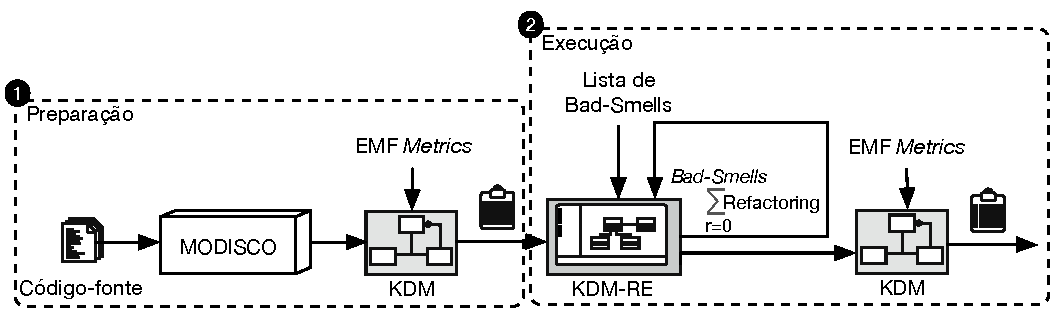
\includegraphics[scale=0.9]{images/Figura_Experimento}
	\fautor
\end{figure}

\subsubsection{Preparação}

Alguns dias antes da realização do experimento, o código-fonte dos sete sistemas apresentado na Tabela~\ref{tab:sistemas_experimentos} foram baixados. Posteriormente, todos esses sete sistemas foram transformados em instâncias do metamodelo KDM. Essa transformação foi realizada por meio da ferramenta MoDisco\footnote{\texttt{https://eclipse.org/MoDisco/}} (ver Figura~\ref{fig:execucao_experimento} \ding{182}). Em seguida, para cada instância do metamodelo KDM gerada (que representa os sete sistemas) a ferramenta EMF \textit{Metrics}~\cite{Arendt_2012, Thorsten_2010_durelli} foi executada. Essa ferramenta foi escolhida para mensurar os atributos de qualidade QMOOD (reusabilidade, flexibilidade, facilidade de compreensão e eficácia). Segundo~\citeonline{Arendt_2012, Thorsten_2010_durelli} EMF \textit{Metrics} é um Eclipse \textit{plug-in} que provê a especificação e calcula métricas para qualquer instância de metamodelo que utilize como base o metamodelo EMF, neste caso o metamodelo KDM. Mais especificadamente EMF \textit{Metrics} calcula as métricas apresentadas na Tabela~\ref{tab:QMOOD_quality_metrics} e em seguida as formulas apresentadas na Tabela~\ref{tab:QMOOD_quality_metrics2} foram mensuradas. Como resultado da aplicação do EMF \textit{Metrics} e da Tabela~\ref{tab:QMOOD_quality_metrics2} uma lista especificando os atributos de qualidade QMOOD (\aspas{reusabilidade}, \aspas{flexibilidade}, \aspas{facilidade de compreensão} e \aspas{eficácia}) foi obtida para os sete sistemas.

\subsubsection{Execução}

Após gerar as instâncias do metamodelo KDM dos sete sistemas e aplicar a ferramenta EMF \textit{Metrics} para mensurar os atributos de qualidade QMOOD, o próximo passo é a aplicação das refatorações no metamodelo KDM por meio da ferramenta KDM-RE (ver Capítulo~\ref{chapter:ferramenta_kdm_re}). Como já salientado, a ferramenta KDM-RE no seu estado atual não identifica \textit{bad-smells}. Dessa forma, um conjunto de artigos foi lido na integra, pois listam e descrevem um conjunto de \textit{bad-smells} dos sete sistemas utilizados nesse experimento~\cite{Kessentini_2011, Ouni_2013, Moha_2010, Kessentini_2010}. Esses artigos apresentam uma lista completa dos \textit{bad-smells} identificados. Essa lista foi utilizada nesse experimento para guiar o engenheiro de modernização a identificar qual refatoração aplicar (ver Figura~\ref{fig:execucao_experimento} \ding{183}).

Após tomar conhecimento dos \textit{bad-smells} de cada sistema um conjunto de refatorações foi escolhido e depois executado por meio da ferramenta KDM-RE. Cada refatoração foi aplicada para tentar resolver e remover os \textit{bad-smells} identificados e melhorar assim os atributos de qualidade QMOOD. As refatorações escolhidas para remover os \textit{bad-smells} e melhorar os atributos de qualidade foram criteriosamente identificadas no catálogo de refatoração proposto por~\citeonline{Fowler1999} que descreve qual (is) refatoração (ões) aplicar para resolver um determinado \textit{bad-smell}. É importante salientar que nesse experimento as refatorações não foram aplicadas no diagrama de classe, ou seja, de forma totalmente manual e por intervenção de \textit{Wizards} como apresentada no Capítulo~\ref{chapter:ferramenta_kdm_re}. As refatorações não foram executadas manualmente pelo engenheiro de software uma vez que muitas refatorações foram aplicadas o que iria demandar muito tempo para a condução do experimento. Dessa forma, foi criado um arquivo que continha as refatorações, os parâmetros e os caminhos para cada instância do KDM que representavam os sete sistemas utilizados no experimento. Esse arquivo foi criado tendo como base os \textit{bad-smell} identificados, assim soube-se previamente qual refatoração aplicar, bem como seus parâmetros – portanto, a ferramenta KDM-RE executou as refatorações de forma semiautomática diminuindo o tempo para a condução do experimento. Para cada refatoração um limite de tempo de 5 minutos foi definido, esse limite de tempo é importante para verificar se a ferramenta KDM-RE não entrou em \textit{loop} infinito.
As refatorações que foram aplicadas nos sete sistemas estão apresentadas na Tabela~\ref{tab:experimento_refatoracoes_aplicadas}, bem como suas respectivas siglas. 



\begin{table}[h]
\centering
\caption{Refatorações aplicadas no experimento 1.}
\label{tab:experimento_refatoracoes_aplicadas}
\begin{tabular}{ | m{3.5cm} | m{1.2cm}|m{2.2cm}| m{1.2cm}|}
\hline
\multicolumn{1}{|c|}{Refatorações} & \multicolumn{1}{c|}{Siglas} & \multicolumn{1}{c|}{Sistemas} & \multicolumn{1}{c|}{Siglas}\\ 
\hline
\multicolumn{1}{|c|}{Move Method} & \multicolumn{1}{c|}{MM} & \multicolumn{1}{c|}{Xerces-J} & \multicolumn{1}{c|}{XJ}\\ 
\hline
\multicolumn{1}{|c|}{Move Field} & \multicolumn{1}{c|}{MF} & \multicolumn{1}{c|}{Jexel} & \multicolumn{1}{c|}{JEX}\\ 
\hline
\multicolumn{1}{|c|}{Extract Class} & \multicolumn{1}{c|}{EC} & \multicolumn{1}{c|}{JFreeChart} & \multicolumn{1}{c|}{JFC}\\ 
\hline
\multicolumn{1}{|c|}{Extract Interface} & \multicolumn{1}{c|}{EI} & \multicolumn{1}{c|}{Jester} & \multicolumn{1}{c|}{JES} \\ 
\hline
\multicolumn{1}{|c|}{Move Class} & \multicolumn{1}{c|}{MC} & \multicolumn{1}{c|}{GanttProject} & \multicolumn{1}{c|}{GP} \\ 
\hline
\multicolumn{1}{|c|}{Pull Up Field} & \multicolumn{1}{c|}{PUF} & \multicolumn{1}{c|}{ArtofIllusion} & \multicolumn{1}{c|}{AOIL} \\ 
\hline
\multicolumn{1}{|c|}{Pull Up Method} & \multicolumn{1}{c|}{PUM} & \multicolumn{1}{c|}{JHotDraw} & \multicolumn{1}{c|}{JHD} \\ 
\hline
\multicolumn{1}{|c|}{Push Down Field} & \multicolumn{1}{c|}{PDF} &\multicolumn{1}{c|}{\textemdash} &\multicolumn{1}{c|}{\textemdash} \\ 
\hline
\multicolumn{1}{|c|}{Push Down Method} & \multicolumn{1}{c|}{PDM} &\multicolumn{1}{c|}{\textemdash} &\multicolumn{1}{c|}{\textemdash} \\ 
\hline
\end{tabular}
\end{table}


Na Tabela~\ref{tab:experimento_dados_refatoracoes_aplicadas} é possível observar os dados relacionados com a quantidade de refatorações aplicada em cada sistema. Nota-se que a refatoração \texttt{Move Method} foi a refatoração mais executada, aproximadamente 26.35\%.  Em seguida, a refatoração \texttt{Move Field} foi a segunda refatoração mais aplicada, aproximadamente 13.42\%. A maioria das refatorações aplicadas está relacionada com mover (\texttt{Move Field} e \texttt{Move Method}) e extrair elementos (\texttt{Extract Class}), somando as refatorações \texttt{Move Method}, \texttt{Move Field} e \texttt{Extract Class} têm-se 51.06\% das refatorações aplicadas – ou seja, mais da metade as refatorações. Esses dados estão diretamente relacionados aos \textit{bad-smells} utilizados nesse experimento: \textit{blob}, \textit{data class} e \textit{spaghetti code}. Por exemplo, para remover o \textit{bad-smell} do tipo \textit{blob} é necessário mover elementos de uma classe para outra classe a fim de reduzir o número de funcionalidades e adicionar comportamento em outras classes. Similarmente para remover o \textit{bad-smell} do tipo \textit{data class} deve-se aplicar a refatoração \texttt{Move Method}. Ainda observando a Tabela~\ref{tab:experimento_dados_refatoracoes_aplicadas} é possível observar que as refatorações menos aplicadas foram: \texttt{Push Up Method}, \texttt{Push Up Field} e \texttt{Move Class}, respectivamente. 

\begin{table}[h]
\centering
\caption{Quantidade de refatorações aplicadas no experimento 1.}
\label{tab:experimento_dados_refatoracoes_aplicadas}
\begin{tabular}{c|c|c|c|c|c|c|c|c|c|}
\cline{2-10}
                                   & \multicolumn{9}{c|}{Sistemas}                                \\ \hline
\multicolumn{1}{|c|}{Refatorações} & XJ & JEX & JFC & JES & GP & AOIL & JHD & Média & Porcentagem \\ \hline
\multicolumn{1}{|c|}{MM}           & 40 & 30  & 45  & 35  & 43 & 45   & 23  & 37.29 & 26.34\%     \\ \hline
\multicolumn{1}{|c|}{MF}           & 25 & 15  & 20  & 16  & 21 & 23   & 13  & 19.00 & 13.42\%     \\ \hline
\multicolumn{1}{|c|}{EC}           & 15 & 20  & 20  & 19  & 12 & 15   & 11  & 16.00 & 11.30\%     \\ \hline
\multicolumn{1}{|c|}{EI}           & 13 & 10  & 15  & 16  & 8  & 12   & 10  & 12.00 & 8.48\%      \\ \hline
\multicolumn{1}{|c|}{MC}           & 9  & 11  & 7   & 13  & 10 & 10   & 18  & 11.14 & 7.87\%      \\ \hline
\multicolumn{1}{|c|}{PUF}          & 12 & 14  & 5   & 8   & 12 & 11   & 9   & 10.14 & 7.16\%      \\ \hline
\multicolumn{1}{|c|}{PUM}          & 10 & 9   & 8   & 6   & 8  & 14   & 13  & 9.71  & 6.86\%     \\ \hline
\multicolumn{1}{|c|}{PDF}          & 17 & 13  & 15  & 10  & 9  & 16   & 8   & 12.57 & 8.88\%      \\ \hline
\multicolumn{1}{|c|}{PDM}          & 16 & 12  & 14  & 11  & 10 & 18   & 15  & 13.71 & 9.69\%      \\ \hline
\end{tabular}
\end{table}


Após a aplicação das refatorações nos sete sistemas a ferramenta EMF \textit{Metrics} foi executada novamente para mensurar os atributos de qualidade QMOOD. A análise dos dados é apresentada na próxima seção.

\subsection{Análise dos Dados do Experimento 1}

Na Tabela~\ref{tab:dados_coletados_experimento_1} é possível observar os dados relacionados aos atributos (reusabilidade, flexibilidade, facilidade de compreensão e eficácia) de qualidade avaliados no experimento 1 antes e após a aplicação das refatorações apresentadas na Tabela~\ref{tab:experimento_dados_refatoracoes_aplicadas}. A Tabela~\ref{tab:dados_coletados_experimento_1} possui sete colunas, \aspas{Antes} representa as métricas mensuradas dos sistemas antes de aplicar as refatorações. \aspas{Depois} representa as métricas coletadas dos sistemas após a aplicação das refatorações e \aspas{Diferença} representa a diferença das colunas \aspas{Antes} e \aspas{Depois}, ou seja, a diferença entre as métricas são calculadas da seguinte forma: \aspas{Depois}-\aspas{Antes}. Os mesmos dados são plotados nos gráficos de barra nas Figuras~\ref{fig:immediate}, \ref{fig:proximal}, \ref{fig:distal} e \ref{fig:combined}. 


\begin{table}[h]
\centering
\caption{Dados coletados do experimento 1.}
\label{tab:dados_coletados_experimento_1}
\begin{tabular}{c|l|l|l|l|l|l|}
\cline{2-7}
\multicolumn{1}{l|}{}               & \multicolumn{3}{c|}{Reusabilidade}             & \multicolumn{3}{c|}{Flexibilidade} \\ \hline
\multicolumn{1}{|c|}{Sistemas}      & Antes         & Depois        & Diferença      & Antes     & Depois    & Diferença  \\ \hline
\multicolumn{1}{|c|}{Xerces-J}      & \multicolumn{1}{c|}{0.061}          & \multicolumn{1}{c|}{0.082}          & \multicolumn{1}{c|}{0.021} & \multicolumn{1}{c|}{0.128}      & \multicolumn{1}{c|}{0.136}      &\multicolumn{1}{c|}{0.008}\\ \hline
\multicolumn{1}{|c|}{Jexel}         & \multicolumn{1}{c|}{0.112}& \multicolumn{1}{c|}{0.124} & \multicolumn{1}{c|}{0.012} & \multicolumn{1}{c|}{0.145}      & \multicolumn{1}{c|}{0.152}      &\multicolumn{1}{c|}{0.007}\\ \hline
\multicolumn{1}{|c|}{JFreeChart}    & \multicolumn{1}{c|}{0.147}& \multicolumn{1}{c|}{0.161}& \multicolumn{1}{c|}{0.014} & \multicolumn{1}{c|}{0.129}      & \multicolumn{1}{c|}{0.143}      & \multicolumn{1}{c|}{0.014} \\ \hline
\multicolumn{1}{|c|}{Jester}        & \multicolumn{1}{c|}{0.072}& \multicolumn{1}{c|}{0.068}& \multicolumn{1}{c|}{-0.004} & \multicolumn{1}{c|}{0.081}      & \multicolumn{1}{c|}{0.094}      & \multicolumn{1}{c|}{0.013}  \\ \hline
\multicolumn{1}{|c|}{GanttProject}  & \multicolumn{1}{c|}{0.089}& \multicolumn{1}{c|}{0.127}          & \multicolumn{1}{c|}{0.038} & \multicolumn{1}{c|}{0.153}      & \multicolumn{1}{c|}{0.178}      &  \multicolumn{1}{c|}{0.025} \\ \hline
\multicolumn{1}{|c|}{ArtofIllusion} & \multicolumn{1}{c|}{0.041}          & \multicolumn{1}{c|}{0.092}          & \multicolumn{1}{c|}{0.051} & \multicolumn{1}{c|}{0.111}      & \multicolumn{1}{c|}{0.136}      & \multicolumn{1}{c|}{0.025} \\ \hline
\multicolumn{1}{|c|}{JHotDraw}      & \multicolumn{1}{c|}{0.028}          & \multicolumn{1}{c|}{0.057}          & \multicolumn{1}{c|}{0.029} & \multicolumn{1}{c|}{0.039}      & \multicolumn{1}{c|}{0.054}      & \multicolumn{1}{c|}{0.015}\\ \hline
\multicolumn{1}{|c|}{Média}         & \multicolumn{1}{c|}{0.078}         & \multicolumn{1}{c|}{0.094}         & \multicolumn{1}{c|}{0.023} & \multicolumn{1}{c|}{0.112}     & \multicolumn{1}{c|}{0.127}     & \multicolumn{1}{c|}{0.015} \\ \hline
\multicolumn{1}{|l|}{Porcentagem}   & 43.62\%       & 56.38\%       &\multicolumn{1}{c|}{12.77\%}                & 46.81\%   & 53.19\%   & \multicolumn{1}{c|}{6.37\%}\\ \hline
                                    & \multicolumn{3}{c|}{Facilidade de Compreensão} & \multicolumn{3}{c|}{Eficácia}      \\ \hline
\multicolumn{1}{|c|}{Sistemas}      & Antes         & Depois        & Diferença      & Antes     & Depois    & Diferença  \\ \hline
\multicolumn{1}{|c|}{Xerces-J}      & \multicolumn{1}{c|}{-0.21}& \multicolumn{1}{c|}{-0.289}          &\multicolumn{1}{c|}{-0.079}&\multicolumn{1}{c|}{0.071}&\multicolumn{1}{c|}{0.082}&\multicolumn{1}{c|}{0.011}            \\ \hline
\multicolumn{1}{|c|}{Jexel}         & \multicolumn{1}{c|}{-0.162}          & \multicolumn{1}{c|}{-0.218}          &\multicolumn{1}{c|}{-0.056} & \multicolumn{1}{c|}{0.052}          & \multicolumn{1}{c|}{0.061}          &\multicolumn{1}{c|}{0.009}            \\ \hline
\multicolumn{1}{|c|}{JFreeChart}    & \multicolumn{1}{c|}{-0.159}          & \multicolumn{1}{c|}{-0.213} &\multicolumn{1}{c|}{-0.054}&\multicolumn{1}{c|}{0.04}&\multicolumn{1}{c|}{0.031}&\multicolumn{1}{c|}{-0.009}\\ \hline
\multicolumn{1}{|c|}{Jester}        & \multicolumn{1}{c|}{-0.143}          & \multicolumn{1}{c|}{-0.236}          &\multicolumn{1}{c|}{-0.093}&\multicolumn{1}{c|}{0.097}&\multicolumn{1}{c|}{0.092}&\multicolumn{1}{c|}{-0.005}\\ \hline
\multicolumn{1}{|c|}{GanttProject}  & \multicolumn{1}{c|}{-0.231}          & \multicolumn{1}{c|}{-0.289}          &\multicolumn{1}{c|}{-0.058}&\multicolumn{1}{c|}{0.046}&\multicolumn{1}{c|}{0.057}&\multicolumn{1}{c|}{0.011}\\ \hline
\multicolumn{1}{|c|}{ArtofIllusion} & \multicolumn{1}{c|}{-0.093}          & \multicolumn{1}{c|}{-0.147}          &\multicolumn{1}{c|}{-0.054}&\multicolumn{1}{c|}{0.032}&\multicolumn{1}{c|}{0.043}&\multicolumn{1}{c|}{0.012}\\ \hline
\multicolumn{1}{|c|}{JHotDraw}             & \multicolumn{1}{c|}{-0.042}          & \multicolumn{1}{c|}{-0.098}          &\multicolumn{1}{c|}{-0.054}&\multicolumn{1}{c|}{0.011}&\multicolumn{1}{c|}{0.022}&\multicolumn{1}{c|}{0.011}\\ \hline
\multicolumn{1}{|c|}{Média}         & \multicolumn{1}{c|}{-0.148}         & \multicolumn{1}{c|}{-0.212}         &\multicolumn{1}{c|}{-0.064}&\multicolumn{1}{c|}{0.049}&\multicolumn{1}{c|}{0.055}&\multicolumn{1}{c|}{0.005}\\ \hline
\multicolumn{1}{|l|}{Porcentagem}   & 41.11\%       & 58.89\%       &\multicolumn{1}{c|}{17.79\%}&  \multicolumn{1}{c|}{47.35\%}  &  \multicolumn{1}{c|}{52.65\%}  &\multicolumn{1}{c|}{5.29\%}\\ \hline
\end{tabular}
\end{table}

Nota-se que todos os atributos de qualidade foram melhorados após a aplicação das refatorações: (\textit{i}) \aspas{reusabilidade} (antes = 43.62\%, depois = 56.38\% e diferença = 12.77\%), \aspas{flexibilidade} (antes = 46.81\%, depois = 53.19\% e diferença = 6.37\%), \aspas{facilidade de compreensão} (antes = 41.11\%, depois = 58.89\% e diferença = 17.79\%) e \aspas{eficácia} (antes = 47.35\%, depois = 52.65\% e diferença = 5.29\%).
É importante observar que o atributo de qualidade \aspas{facilidade de compreensão} foi o que alcançou o maior ganho, aproximadamente 59\%. Por outro lado, o atributo de qualidade \aspas{eficácia} teve o menor ganho, alcançando aproximadamente 53\%. Isto deve-se principalmente as refatorações aplicadas. Por exemplo, a maioria das refatorações aplicadas (\texttt{Move Method}, \texttt{Move Field} e \texttt{Extract Class} (ver Tabela~\ref{tab:experimento_dados_refatoracoes_aplicadas})) aumentam o acoplamento (DCC), coesão (CAM) e tamanho do projeto (DSC) que são métricas utilizadas para calcular o atributo de qualidade Facilidade de Compreensão.

Além disso, pode-se também observar nas Figuras~\ref{fig:immediate}, \ref{fig:proximal}, \ref{fig:distal} e \ref{fig:combined} que o sistema JHotDraw produziu o menor aumento para os quatro atributos de qualidade. Acredita-se que a principal razão é que JHotDraw é conhecido na literatura por seguir as melhores práticas de projeto e implementação~\cite{Kessentini_2010}, assim, poucas refatorações foram aplicadas nesse sistema.



\begin{figure}[!h]    
\begin{minipage}[h]{0.5\textwidth}
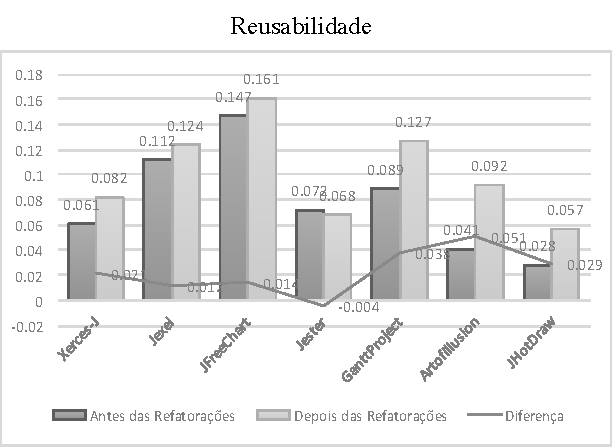
\includegraphics[width=\linewidth]{images/GraficoBarraExperimentoReusabilidadeNovo}
\caption{Reusabilidade antes e depois das refatorações.}
\label{fig:immediate}
\end{minipage}
\hspace{\fill}
\begin{minipage}[h]{0.5\textwidth}
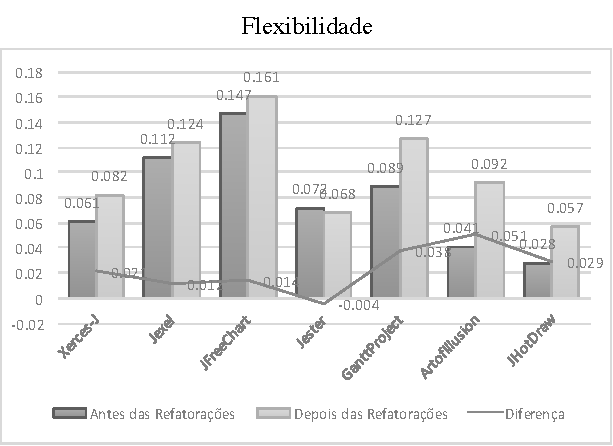
\includegraphics[width=\linewidth]{images/GraficoBarraExperimentoFlexibilidadeNovo}
\caption{Flexibilidade antes e depois das refatorações.}
\label{fig:proximal}
\end{minipage}

\vspace*{0.5cm} % (or whatever vertical separation you prefer)
\begin{minipage}[h]{0.5\textwidth}
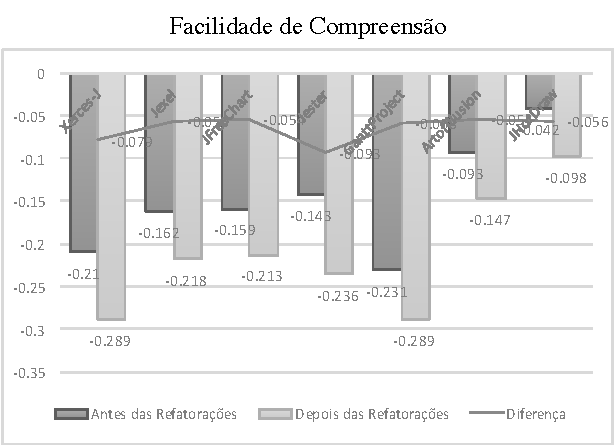
\includegraphics[width=\linewidth]{images/GraficoBarraExperimentoFacilidadeDeCompreensaoNovo}
\caption{Facilidade de Compreensão antes e depois das refatorações.}
\label{fig:distal}
\end{minipage}
\hspace{\fill}
\begin{minipage}[h]{0.5\textwidth}
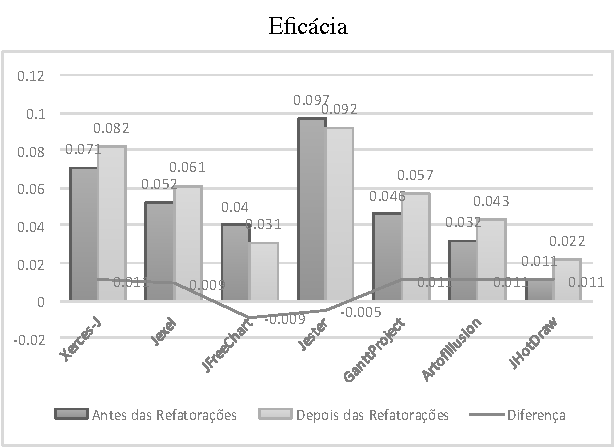
\includegraphics[width=\linewidth]{images/GraficoBarraExperimentoEficaciaNovo}
\caption{Eficácia antes e depois das refatorações.}
\label{fig:combined}
\end{minipage}

\end{figure}

\begin{figure}[h]
	\centering
	\caption{Gráficos resultantes do teste de normalidade.}
	\label{fig:qq_plot_experimento1}
	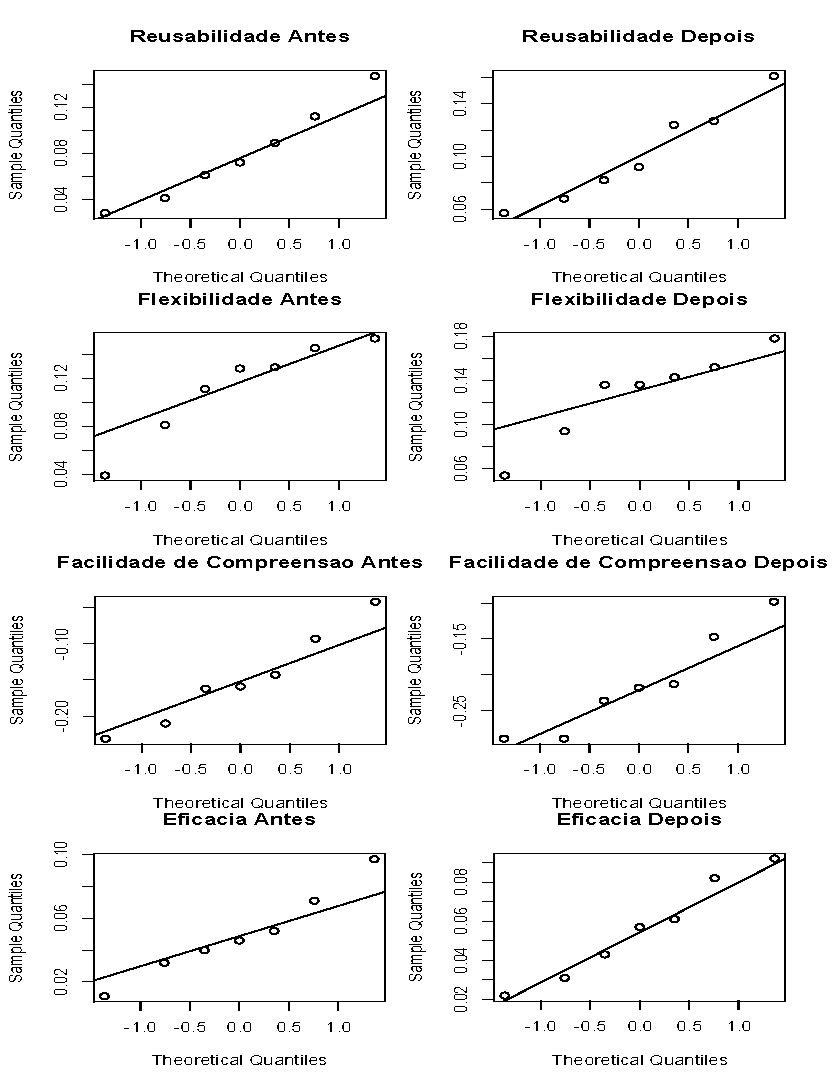
\includegraphics[scale=0.9]{images/qqPlotAll2_experimento1}
	\fautor
\end{figure}

\subsubsection{Teste das Hipóteses}

Nesta seção são apresentados os resultados dos testes estatísticos aplicados sobre os dados coletados no experimento. Antes de aplicar qualquer teste estatístico é importante verificar se um conjunto de dados segue, ou não, uma distribuição normal (ver Seção~\ref{sec:shapiro_wilk}). Dessa forma, para os conjunto de dados (antes e depois das refatorações) dos atributos de qualidade \aspas{reusabilidade}, \aspas{flexibilidade}, \aspas{facilidade de compreensão} e \aspas{eficácia} apresentados na Tabela~\ref{tab:dados_coletados_experimento_1} aplicou-se o teste \textbf{Shapiro-Wilk} para verificar se os dados seguem uma distribuição normal. Além disso, para cada conjunto de dados também foi criado gráficos de probabilidade denominado \textit{Q-Q Plot}, ver Figura~\ref{fig:qq_plot_experimento1}. Como pode ser observado na Tabela~\ref{tab:dados_coletados_experimento_1} o p-valor resultante para cada atributo de qualidade é: reusabilidade (antes = 0.8988, depois = 0.7245), flexibilidade (antes = 0.3298, depois = 0.416), facilidade de compreensão (antes = 0.8137, depois = 0.4716) e eficácia (antes = 0.9355, depois = 0.8362). Note que todos os p-valor dos testes foram superior a 0.05, então, pode-se afirmar, com nível de confiança de 95\%, que os dados seguem uma distribuição normal. Isso também pode ser verificado nos gráficos mostrados na Figura~\ref{fig:qq_plot_experimento1}. Nota-se que em tais gráficos os pontos estão formados pelo quantis amostrais e o pontos alinham-se nas respectivas retas, assim, pode-se afirmar que os dados estão normalizados.

Como os dados estão normalizados (ver Tabela~\ref{tab:shapiro_experimento_1}), o \textit{Paried T-Test} foi aplicado sobre os dados para verificar as hipóteses da \mathbf{$QP_1$} do experimento (Seção~\ref{sec:experimento}). Como mostrado na Tabela~\ref{tab:experimento_1_10_15} o todos os atributos de qualidade foram p-valor < 0.05, então, como nível de confiança de 95\%, existem evidências de diferença entre os atributos de qualificação antes e após a aplicação das refatorações. Portanto, pode-se refutar as hipóteses nulas \textbf{$H1_{0}$}, \textbf{$H2_{0}$} e \textbf{$H3_{0}$} e as hipóteses alternativas foram aceitas. O atributo de qualidade eficácia tem uma relação com o atributo de qualidade facilidade de compreensão - quando um é melhorado o outro tende a piorar. Dessa forma, para o atributo de qualidade eficácia não pode-se refutar a hipótese nula, os dados não se demostraram estatisticamente significantes para refuta-la, ou seja, não houve evidência suficientemente forte para provar que a hipótese nula era falsa.

\begin{table}[]
\centering
\caption{\textit{Shapiro-Wilk} aplicado para verificar se os dados seguem uma distribuição normal.}
\label{tab:shapiro_experimento_1}
\begin{tabular}{|c|c|c|c|}
\hline
\multicolumn{4}{|c|}{Reusabilidade}                       \\ \hline
\multicolumn{2}{|c|}{Antes} & \multicolumn{2}{c|}{Depois} \\ \hline
w=0.97        & p-valor=0.8988        & w=0.9494        & p-valor=0.7245        \\ \hline
\multicolumn{4}{|c|}{Flexibilidade}                       \\ \hline
\multicolumn{2}{|c|}{Antes} & \multicolumn{2}{c|}{Depois} \\ \hline
w=0.8998        & p-valor=0.3298        & w=0.9129        & p-valor=0.416        \\ \hline
\multicolumn{4}{|c|}{Facilidade de Compreensão}           \\ \hline
\multicolumn{2}{|c|}{Antes} & \multicolumn{2}{c|}{Depois} \\ \hline
w=0.9594        & p-valor=0.8137        & w=0.9203        & p-valor=0.4716         \\ \hline
\multicolumn{4}{|c|}{Eficácia}                            \\ \hline
\multicolumn{2}{|c|}{Antes} & \multicolumn{2}{c|}{Depois} \\ \hline
w=0.9756        & p-valor=0.9355         & w=0.9621        & p-valor=0.8362        \\ \hline
\end{tabular}
\end{table}


\begin{table}[]
\centering
\caption{\textit{Paried T-Test} aplicado sobre os dados para verificar as hipóteses da \mathbf{$QP_1$}.}
\label{tab:experimento_1_10_15}
\begin{tabular}{|m{1cm}|l|l|m{7.1cm}|}
\hline
\multicolumn{1}{|c|}{Atributo de Qualidade} & \multicolumn{1}{c|}{T} & \multicolumn{1}{c|}{P-valor} & \multicolumn{1}{c|}{Comentário} \\ \hline
\multicolumn{1}{|c|}{Reusabilidade} & \multicolumn{1}{c|}{-3.3498} & \multicolumn{1}{c|}{0.01542} & Refuta-se \textbf{$(H1_{0})$} com significância de 5\%\\ \hline
\multicolumn{1}{|c|}{Flexibilidade} &\multicolumn{1}{c|}{-5.5602}& \multicolumn{1}{c|}{0.001433} &Refuta-se \textbf{$(H2_{0})$} com significância de 5\%\\ \hline
\multicolumn{1}{|c|}{Facilidade de Compreensão} & \multicolumn{1}{c|}{11.0194} &    \multicolumn{1}{c|}{3.322e-05}&Refuta-se \textbf{$(H3_{0})$} com significância de 5\%\\ \hline
\multicolumn{1}{|c|}{Eficácia}&\multicolumn{1}{c|}{-1.6951}&\multicolumn{1}{c|}{0.141}&\multicolumn{1}{c|}{Não refuta-se \textbf{$(H4_{0})$}, pois 0.141 > 0.05}\\ \hline
\end{tabular}
\end{table}

\subsection{Ameaças à Validade do Experimento 1}

Nesta seção são apresentados os itens que podem afetar os valores e a conclusão do experimento 1. O experimento 1 é afetado pelas ameaças à validade listadas abaixo.

\textbf{Validade Externa:} Validade Externa refere-se a generalidade do experimento. O experimento 1, foi conduzido em sete sistemas diferentes de código aberto amplamente utilizados, pertencentes a diferentes domínios e com tamanhos diferentes. No entanto, não é possível afirmar que os resultados podem ser generalizados para todas as aplicações Java instanciadas para o metamodelo KDM, bem como outras linguagens de programação, e outros engenheiros de software. Outra ameaça pode ser o número limitado de sujeitos/sistemas estudados, o que ameaça externamente a generalização dos nossos resultados. Replicações futuras deste estudo são necessárias para confirmar o resultado da abordagem.


\textbf{Validade por Construção}: A validade de construção está preocupada com a relação entre a teoria e o que é observado. Como a ferramenta KDM-RE no seu estado atual não identifica \textit{bad-smells} a escolha das refatorações aplicadas esta totalmente dependente do conhecimento de terceiros. Dessa forma, para mitigar essa ameaça, os sete sistamas foram escolhidos, pois já haviam identificados e listados os \textit{bad-smells} na literatura por outros autores~\cite{Kessentini_2011, Ouni_2013, Moha_2010, Kessentini_2010}.

\textbf{Validade de Conclusão}: Essa validade está relacionada com a precisão das métricas empregadas durante o experimento 1. Para mitigar essa ameaça, foi-se utilizado métricas já consolidadas na literatura, tais como QMOOD. 


\section{Experimento 2: Ferramenta KDM-RE}\label{sec:experimento_KDM_re}

Nesta seção é apresentado um experimento conduzido com o objetivo de analisar o uso da ferramenta KDM-RE (ver Capítulo X\change{mudar}) durante a aplicação de refatorações para o metamodelo KDM. Para atingir esse objetivo, foi realizada uma comparação entre as ferramentas KDM-RE e EMF Refactor\footnote{\texttt{https://www.eclipse.org/emf-refactor/}}.

\subsection{Definição e Planejamento do Experimento 2}

Esse experimento foi definido utilizando o modelo GQM~\cite{Wohlin} e foi dividido em cinco partes:

\begin{itemize}
\item \textbf{Objeto de estudo}: o objeto de estudo desse experimento é a ferramenta KDM-RE;
\item \textbf{Propósito}: o propósito desse experimento é avaliar a ferramenta KDM-RE;
\item \textbf{Perspectiva}: esse experimento esta sendo executado sobre a perspectiva de desenvolvedores;
\item \textbf{Qualidade de foco}: o efeito primário sobre investigação nesse experimento são eficiência (tempo) e à facilidade de uso da ferramenta KDM-RE;
\item \textbf{Contexto}: esse experimento foi conduzido utilizando Eclipse 4.3.2 em uma máquina 2.5 GHz Intel Core i5 com 8GB de memória física executando o sistema operacional Mac OS X 10.9.2.
\end{itemize}

O experimento pode ser resumido utilizando o seguinte \textit{template}~\cite{Wohlin}:

\textbf{Analisar} a ferramenta KDM-RE

\textbf{Com o propósito de} avaliação

\textbf{Com respeito à} eficiência (tempo) e à facilidade de uso

\textbf{Do ponto de vista dos} desenvolvedores

\textbf{No contexto de } de estudantes de mestrado e de doutorado dos cursos de Ciência da Computação da Universidade de São Paulo (USP-ICMC) e da Universidade Federal de São Carlos (UFSCar).

\subsection{Contexto e Participantes}

O contexto desse experimento foi \textbf{multi-teste dentro de um objeto de estudo}~\cite{Wohlin}, uma vez que foi consistituído de testes experimentais executados por um grupo de indivíduos para estudar uma única abordagem, que é a ferramenta KDM-RE. O experimento foi realizada em um laboratório de computação no ambiente universitário. Ao todo, participaram 20 alunos (sujeitos) dos cursos de mestrado e doutorado em Ciência da Computação da USP-ICMC e UFSCar. Todos tinham experiência prévia em desenvolvimento de software e alguns deles já haviam realizado refatoração de sistemas Java utilizando os recursos fornecidos pelo Eclipse IDE.

\subsubsection{Formulação das Hipóteses}

As seguintes questões, métricas e hipóteses foram definidas para esse experimento:

\textbf{Questão de Pesquisa 2.1} (\textbf{$QP_{2.1}$}): Qual ferramenta propicia a aplicação de refatorações em instâncias do metamodelo KDM em termos de tempo?

\begin{itemize}
\item \textbf{Métrica 2.1} (\textbf{$M_{2.1}$}): tempo (\textit{t}) gasto pelos sujeitos para aplicar refatorações em instâncias do metamodelo KDM.
\begin{itemize}
\item \textbf{Hipótese Nula} (\textbf{$H2.1_0$}): Não há diferença significativa no tempo gasto pelos participantes durante a aplicação de refatorações em instâncias do metamodelo KDM, seja utilizando a ferramenta KDM-RE ou a EMF Refactor. Isso Pode ser formalizado como $t_{KDM-RE} = t_{EMF Refactoror}$
\item \textbf{Hipótese Alternativa} (\textbf{$H2.1_1$}): Há diferença significativa no tempo gasto pelos participantes durante a aplicação de refatorações em instâncias do metamodelo KDM, seja utilizando a ferramenta KDM-RE ou a EMF Refactor. Isso Pode ser formalizado como $t_{KDM-RE} \neq t_{EMF Refactoror}$
\end{itemize}
\end{itemize}

\textbf{Questão de Pesquisa 2.2} (\textbf{$QP_{2.2}$}): Qual ferramenta é mais fácil de ser utilizada?

\begin{itemize}
\item \textbf{Métrica 2.2} (\textbf{$M_{2.2}$}): dificuldades e facilidades citadas pelos participantes sobre cada ferramenta.
\begin{itemize}
\item \textbf{Hipótese Nula} (\textbf{$H2.2_0$}): De acordo com os participantes, não há diferença significativa entre as ferramentas quanto à facilidade de uso. Isso pode ser formalizado como: $f_{KDM-RE} = f_{EMF Refactoror}$ 

\item \textbf{Hipótese Alternativa} (\textbf{$H2.2_1$}): De acordo com os participantes, há diferença significativa entre as ferramentas quanto à facilidade de uso. Isso pode ser formalizado como: $f_{KDM-RE} \neq f_{EMF Refactoror}$
\end{itemize}
\end{itemize}

\subsubsection{Variáveis}

Esse experimento teve as seguintes variáveis independentes: (\textit{i}) o Eclipse IDE versão 4.3.2 com a KDM-RE instalada, (\textit{ii}) a ferramenta EMF Refactor instalada, (\textit{iii}) os sistemas para aplicar as refatorações: (\textit{iii.a}) LabSys (\textit{Laboratory System}) que é um sistema utilizado pela Universidade Federal de Tocantins (UFT) para controlar o uso de laboratórios e (\textit{iii.b}) SIGA (\textit{Integrated System of Academic Management}) que é um sistema utilizado pela UFSCar para realizar todo o controle acadêmico.

As variáveis dependentes são as seguintes: (\textit{i}) eficiência, que está relacionada ao tempo gasto para a aplicação de refatorações nos sistemas LabSys e SIGA e (\textit{ii}) usabilidade, relacionada à opinião dos participantes.

\subsubsection{Modelo}
 
O modelo de experimento utilizado foi \textbf{um fator com dois tratamentos pareados}~\cite{Wohlin}. Nesse experimento, o \textbf{fator} foi a ferramenta utilizada para aplicar refatorações em instâncias do metamodelo KDM, enquanto que os \textbf{tratamentos} foram as ferramentas utilizadas: KDM-RE e EMF Refactor. 

O experimento seguiu o formato em que os participantes são alocados em grupos homogêneos para que o nível de experiência deles são impactasse nos resultados. um Formulário de Caracterização de Participantes (Apêndice X\change{mudar}) foi distribuído para determinar o nível de experiência de cada participante. Nesse formulário os participantes tinham de responder questões de múltipla escolha a respeito do conhecimento deles sobre: \textit{i} linguagem de programação, (\textit{ii}) Eclipse IDE, (\textit{iii}) refatoração, (\textit{vi}) MDD, (\textit{v}) KDM-RE e (\textit{vi}) EMF Refactor. Cada questão possuía a seguinte pontuação: 0, quando o participante não tinha conhecimento algum; 1, quando o participante tinha apenas conhecimento teórico e 2, quando o participante tinha conhecimento teórico e prático.

Os participantes foram treinadas no uso das duas ferramentas utilizadas no experimento. A EMF Refactor foi selecionada porque, assim como a KDM-RE, pode ser utilizada no contexto de qualquer  metamodelo definidos com base no EMF. Além disso, essa ferramenta possui vídeos e tutoriais explicando como utiliza-la. 

Foi decidido que os participantes seriam divididos em dois grupos\textbf{G1} e \textbf{G2}, respectivamente. Também teve-se a preocupação de balancear os grupos. Assim, cada grupo ficou com o mesmo número de participantes que obtiveram pontuação baixa (0-2), média (3-5) e alta (6-8) no Formulário de Caracterização de Participante. Na Tabela~\ref{tab:agrupamento_experimento2} é apresentado como faram definidas as atividades de refatoração para cada um dos participantes do \textbf{G1} e do \textbf{G2}.


\begin{table}[h]
\centering
\caption{Atividade do Experimento 2}
\label{tab:agrupamento_experimento2}
\begin{tabular}{|c|c|c|c|}
\hline
\multirow{2}{*}{Atividade} & \multirow{2}{*}{Sistemas para Refatorar} & \multicolumn{2}{c|}{Ferramenta} \\ \cline{3-4} 
                           &                                          & Grupo 1 (G1)   & Grupo 2 (G2)   \\ \hline
1                          & LabSys                                   & KDM-RE        & EMF Refactor   \\ \hline
2                          & SIGA                                     & EMF Refactor   & KDM-RE         \\ \hline
\end{tabular}
\end{table}

Quando fossem utilizar as ferramentas os participantes tinha que realizar dois passos: (\textit{i}) obter os sistemas já instanciados para o metamodelo KDM e (\textit{ii}) identificar onde aplicar as refatorações a partir de acordo com uma lista já explicando qual refatoração deveria ser realizada, bem como o mecanismo da refatoração. Esse segundo passo foi necessário pois a aplicação de refatorações pode ser uma atividade subjetiva, fazendo com que cada participante demore mais ou menos dependendo da sua escolha. Assim, foi decidido guiar os participantes durante a aplicação das refatorações. 

\subsubsection{Instrumentação}

Os participantes receberam os seguintes materiais para a execução do experimento: (\textit{i}) documentação sobre as refatorações que deveriam ser executadas, (\textit{ii}) manuais da ferramenta KDM-RE e EMF Refactor, (\textit{iii}) um documento com a descrição das refatorações a serem realizadas com cada ferramenta, e o Formulário de Coleta de Dados (Apêndice x\change{mudar}) que os participantes preenchiam o tempo gasto na aplicação das refatorações.


\subsection{Operação do Experimento 2}

Depois definir e planejar o experimento 2, sua fase de operação foi realiza em duas etapas: Preparação e Execução.

\subsubsection{Preparação}

Uma semana antes da execução do experimento os participantes foram treinados com o uso da KDM-RE e da EMF Refactor. Eles também preencheram o Formulário de Caracterização de Participante (Apêndice x\change{mudar}), reportando sua experiência com relação aos conceitos utilizados no experimento. Um experimento piloto também foi realiza para que os participantes obtivessem experiência com a realização das atividades do experimento.

\subsubsection{Execução}

Para a execução do experimento, primeiramente, os participantes foram colocados nos grupos de acordo com a sua pontuação obtida a partir do Formulário de Caracterização de Participante (Apêndice B). Cada grupo ficou com 10 participantes no total. O \textbf{G1} ficou 6 participantes com a pontuação média (3-5) e 4 com pontuação alta (6-8). O \textbf{G2} ficou com 5 participantes com a pontuação média (3-5) e 5 com a pontuação alta (6-8). Após a formação dos grupos os participantes receberam o material para executarem as atividades. O tempo limite foi de 60 minutos para cada uma das atividades.


Na Atividade 1, os participantes aplicaram seis refatorações no sistema LabSys. As refatorações escolhidas para esse experimento foram: \texttt{Extract ClassUnit}, \texttt{Move MethodUnit}, \texttt{Move StorableUnit}, \texttt{Pull Up StorableUnit}, \texttt{Pull Up MethodUnit}, \texttt{Push Down MethodUnit}. O grupo \textbf{G1} utilizou a ferramenta KDM-RE e o grupo \textbf{G2} utilizou a EMF Refactor. Cada participante realizou as suas atividades individualmente e cronometrou o tempo gasto para a aplicação de cada refatoração, separadamente.

A Atividade 2 foi executada da mesma forma que a Atividade 1, todas as seis refatorações também foram aplicadas no sistema SIGA. Porém, agora os participantes do grupo \textbf{G1} utilizaram a EMF Refactor e os do grupo \textbf{G2} utilizaram a KDM-RE. Novamente, cada participante realizou as refatorações individualmente e cronometrou o tempo gasto para a aplicação de cada refatoração.

\subsection{Análise dos Dados do Experimento 2}

\section{Considerações Finais}\label{sec:consideracoes_finais_experimento}